\section{State of the Art}

\subsection{Semantic Segmentation}\label{sec:semantic-segmentation}

The segmentation of wounds belongs to the class of semantic segmantation problems, where a pixel-wise classification is performed. In the case of wound segmentation there are two classes: foreground, which is the wound, and background. Deep Learning methods became dominant in the last years because they became more accessible. Fully Convolutional Neural Networks (fCNN) as a starting point in research had the drawback of resulting in a low output resolution and multiple techniques were invented to increase the output resolution \cite{Litjens2017}. This results in an encoder-decoder architecture as base for the networks, inspired by auto-encoders \cite{linknet}, where the encoder subsamples and the decoder upsamples \cite{Norelyaqine2023}. In such architectures the encoder generates context information, information in the feature space while the decoder maps this information into the spatial context.

Pre-training for such models requires a huge amount of data. A typical data set for such pre-training is the ImageNet object classification data set \cite{SegNet}.

In this project, four different segmentation models are used: U-Net, Linknet, FPN and PSPNet. All are improved architectures about a basic fCNN. Each architecture is described in detail to understand challenges and approaches of localizing information in space.

\paragraph{U-Net}

U-Net is a convolutional network developed for Biomedical Image Segmentation, based on an encoder-decoder architecture. Encoder and decoder are called contracting and expansive path in the original paper, describing their function. They are also described as context path and spatial path \cite{MO2022626}. Both, encoder and decoder consist of different steps to encode and decode the image on different spatial levels. The encoder is a classical CNN; each step consists of two convolutions and a max pooling operation for downsampling. The decoder step upsamples the feature map followed by a convolution. The result is then concatenated with the corresponding feature map from the encdoer path and convolution is applied again. In the final layer, 1x1 convolution is used to map the feature vector to the desired number of classes. This architecture is visualised in figure \ref{fig:unet-architecture}. \cite{unet}

\begin{figure}[htb!]
	\centering
	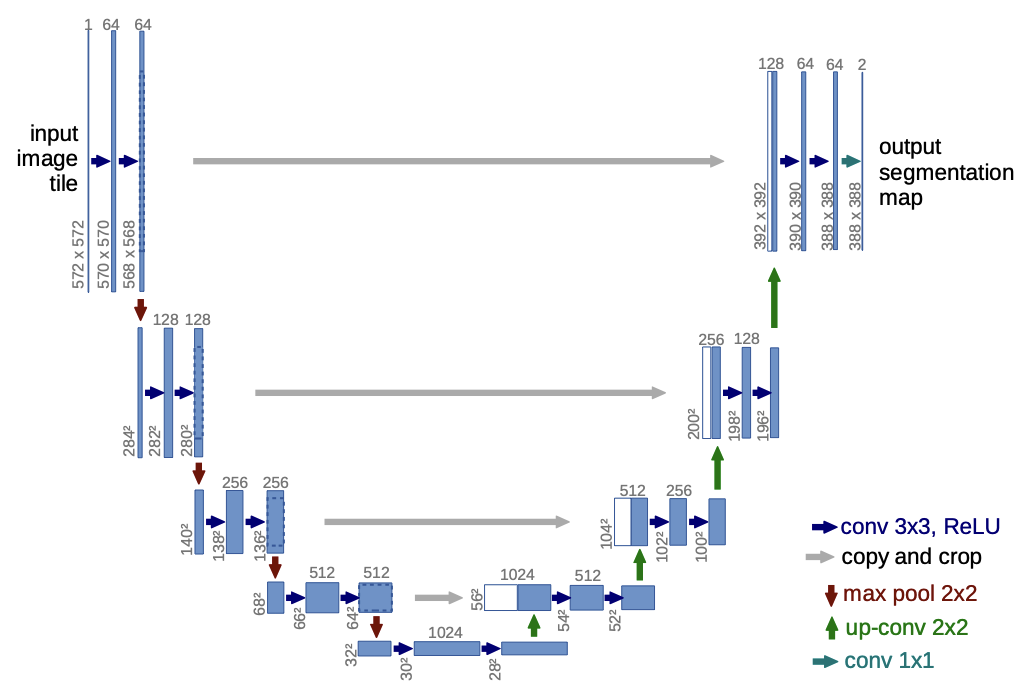
\includegraphics[width=0.8\textwidth]{fig/unet-architecture.png}
	\caption{U-Net architecture for 32x32 pixels in the lowes resolution. Blue boxes are feature maps with the number of feature-channels on top of the boxes and the size shown on the left size. Operations are indicated by the arrows. The skip connections are a concatenation. The figure originally create by \citeauthor{unet} \cite{unet}.}
	\label{fig:unet-architecture}
\end{figure}

The skip connections, connecting the different levels of encoder and decoder prevent a loss of information and extracting the features at different resolutions to retrieve spatial information. By doing this, it is one of the first architectures improving the classical fCNN for semantic segmantation \cite{Litjens2017}. While U-Net provides spatial localization of features, its ability to generalize to multi-scale information is limited \cite{Norelyaqine2023}.

One restriction is, that the input size must be chosen such that all 2x2 max-pooling operations in the encoder are applied to an even x and y size.


\paragraph{Linknet}

Similar to U-Net, Linknet contains of an encoder block for downsampling and a decoder block for upsampling. The downsampling is not done by max pooling as it is in the U-Net architecture but by using a stride of 2 in a convolutional layer. Also does the inital encoder block differ from the following blocks as it uses a larger kernel and uses max pooling. The decoder blocks upsample by a factor of 2 in each block. The final block differs again from the previous blocks. The main difference to the U-Net architecture is how the skip connections are used: Similarly to the U-Net, there are skip connections between the corresponding steps of encoder and decoder, but the feature map from the encoder is not concatenated but added to decoder data. The linknet architecture is visualised in figure \ref{fig:linknet-architecture}. \cite{linknet}

\begin{figure}
	\centering
	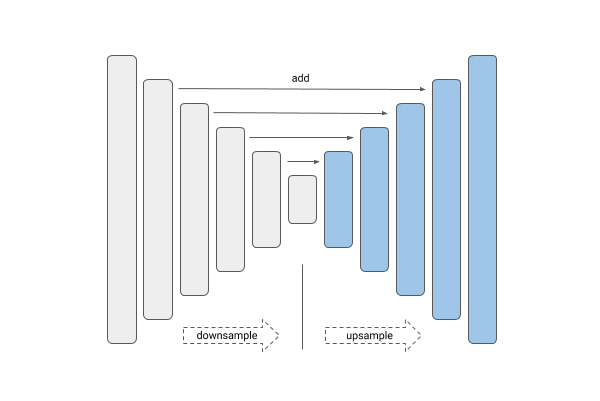
\includegraphics[width=0.5\textwidth]{fig/linknet-architecture.png}
	\caption{A visualisation of the LinkNet architecture originally provided by \citeauthor{SegmentationModels} \cite{SegmentationModels}.}
	\label{fig:linknet-architecture}
\end{figure}


%\begin{itemize}
%	\item "LinkNet sends spatial information directly from the encoder to the matching decoder, conserving as much of the image’s spatial information as feasible."
%	\item "directly connects shallow feature map in encoder module to the decoder module of the corresponding size" $\rightarrow$ accurate position information on shallow layer, avoids redundant parameters and computations \cite{Norelyaqine2023}
%\end{itemize}

The implementation used in this project has four skip connections instead of the original three \cite{SegmentationModels}. Similarly to the U-Net, the input size is restricted such that every upsampling operations need to be applied to an even x and y size.

Linknet has been shown to achieve better results than U-Net under similar conditions \cite{Gao2022}.

\paragraph{FPN}

The Feature Pyramid Network (FPN) architecture creates feature maps of various sizes in multiple layers \cite{Norelyaqine2023}. Similar to the other architectures in consists of an encoder and a decoder, called bottom-up and top-down pathway here\cite{fpn}. Similarly to U-Net, feature maps at different scales with a scaling step of 2 are created in the encoder \cite{fpn}. In the decoder, the feature maps are upsampled and combined with the encoder information of the same level. Similarly to LinkNet, addition is used in the skip connections, but an 1x1 convolution is applied. By doing this so-called feature pyramids are build, containing features at different resolution. \citeauthor{kirillov2019panoptic} proposed a method to use these feature pyramids to obtain a segmentation by merging the feature maps using addition or concatenation \cite{kirillov2019panoptic, SegmentationModels}. The architecture is visualised in figure \ref{fig:fpn-architecture}.

\begin{figure}
	\centering
	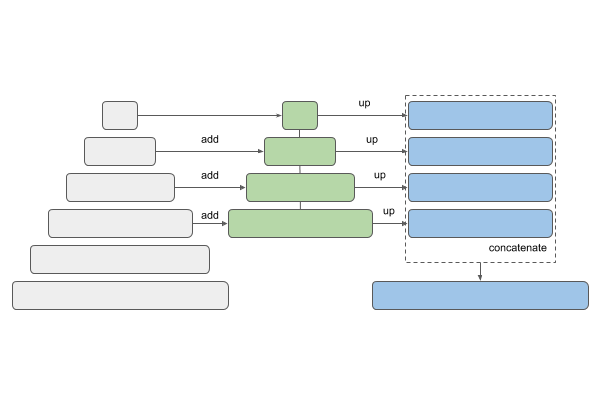
\includegraphics[width=0.6\textwidth]{fig/fpn-architecture.png}
	\caption{A visualisation of the FPN architecture originally provided by \citeauthor{SegmentationModels} \cite{SegmentationModels}. Note, that the feature maps can combined either by concatenation or addition.}
	\label{fig:fpn-architecture}
\end{figure}


\paragraph{PSPNet}

The main part of the Pyramid Scene Parsing Network (PSPNet) is the pyramid pooling module, visualised in part c of figure \ref{fig:pspnet-architecture}, which extracts context information at different scales. A feature map extracted with a pre-trained backbone is pooled at different pyramid scales. This means that global pooling and sub-regions on different locations are used to extract features from a global to a more fine-grained scale. Each of those scales is as passed through a 1x1 convolution and afterwards upsampled to the size of the original feature map. All feature maps including the original feature map from the backbone are concatenated and used to extract the final prediction. By this features on different scales are combined. \cite{Zhao2017, ArcGIS}

\begin{figure}
	\centering
	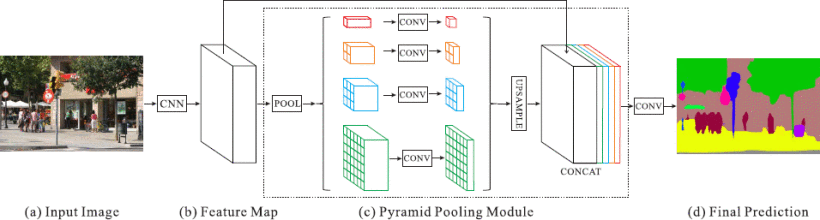
\includegraphics[width=\textwidth]{fig/pspnet-architecture.png}
	\caption{TODO. Originally created by \citeauthor{Zhao2017} \cite{Zhao2017}.}
	\label{fig:pspnet-architecture}
\end{figure}

\subsubsection{Evaluation}

There exist several methods to evaluate how good a predicted segmentation is. Since semantic segmentation performs a pixel-wise classification, resulting in a segmentation mask, classical metrics such as accuracy and precision are available. Two performance metrics that are commonly used in semantic segmentation in medical imaging are the Dice Coefficient and the Intersetcion over Union (IoU) score. They indicate the segmentation quality better than pixel-wise accuracy \cite{Eelbode}.

\paragraph{IOUScore}

The IoU-Score (Intersection over Union), also known as the Jaccard index $J$ describes the ratio between the intersection of the ground truth mask $y$ and the predicted mask $\tilde{y}$ and the union of the predicted and the ground truth mask. By this it compares the similarity of the two masks \cite{Cho2021WeightedIO}.

\begin{align}
	\text{IoU}(y, \tilde{y} :&= \frac{\text{Area of overlap}}{\text{Area of union}}\\
	&=\frac{|y \cap \tilde{y}|}{|y \cup \tilde {y}|}
\end{align}


\paragraph{Dice Coefficient}

The Dice coefficient is the F1 score calclulated for the image masks. In terms of intersection and union, this means it calculates the ratio between two times the overlap between ground truth $y$ and predicted mask $\tilde{y}$ and the total area.

\begin{align}
	\text{Dice}(y, \tilde{y}) :&= 2 \cdot \frac{\text{Area of overlap}}{\text{Total area}}\\
	&= 2 \cdot \frac{|y \cap \tilde{y}|}{|y| + |\tilde{y}|}
\end{align}

To gain more insight into the type of the errors the model makes, the rate of false positives and false negatives can be used do differentiate Type I and Type II errors \cite{DFUC2022}.

% "The difference between the two metrics is that the IoU penalizes under- and over-segmentation more than DSC"

\subsubsection{Loss function}

\begin{itemize}
	\item loss function often uses pixel-wise (weighted) cross-entropy loss even though differentiable approximations of the two metrics exist \cite{Eelbode}
\end{itemize}

% DiceLoss is used in the code

\subsubsection{Data Augmentation}

Data Augmentation is a useful technique to make trained models more robust and accurate. This is especially the case if available data is limited, as the data set size can be either increased or the data set can be made more diverse.

For images, there exist several different possible augmentations. First of all, there are different positional augmentations, including cropping, flipping, rotating and resizing the image. Another class of augmentations are color augmentations, changing the brightness, contrast and saturation of the image. Other augmentations include blurring and dropouts.

Not every augmentation is appropriate for every application. Rotating images of standing animals by 180 degrees for example would not make sense, while rotating images of wounds is appropriate. Therefore, augmentations must be chosen carefully depending on the application.


% https://nanonets.com/blog/data-augmentation-how-to-use-deep-learning-when-you-have-limited-data-part-2/
% https://www.v7labs.com/blog/data-augmentation-guide


\subsection{Wound Segmentation}


As already discussed in the motivation of this project, wound segmentation is a complex problem due to wound characteristics such as different tissues and therefore edges in a wound itself on one side and technical reasons such as e.g. varying lightning, distance to the wound and different angles. 

Before Deep Learning became easily accessible and popular, methods based on features describing color and textures, region growing and optimal thresholding algorithms and classical machine learning models were used to perform segmentation \cite{Scebba2022}. Convolutional Neural Networks replaced manually extracted features by autonomously learned ones \cite{Scebba2022}. Some methods included pre-processing steps to remove the background by e.g. user interaction indicating the background, using a standardized background when taking the image or using manual feature engineering to detect the background more efficiently and make the wound segmentation task easier. Such non-automatic steps limit the use of the segmentation algorithms because they either require more ressources in the image taking process, in the segmentation process or are specifically tailored for specific conditions of lighting or camera settings.

The Diabetic Foot Ulcer Challenge 2022 used FCN, U-Net and SegNet with different backbones and categorical cross-entropy loss as baseline for their challenge, indicating those methods reflect the current state of the art that needs to be improved \cite{DFUC2022}. Generally, such classic models are commonly used and extended with minor adaptions. Two methods stood out in the performed literature review, including more sophisticated adaptions.

\citeauthor{Scebba2022} proposed a method consisting of two steps: An object detection step that produces bounding boxes containing the wounds and a second step that performs segmentation on those areas. Segmentation itself is performed using classical architectures for semantic segmentation as described in section \ref{sec:semantic-segmentation}. The loss function used was pixel-wise weighted binary cross entropy loss. Weighting was calculated based on the number of wound and background pixels of each training set fold.
%TODO: make say why i did not consider this approach

\citeauthor{Oota_2023_WACV} claim they set a new state of the art for wound segmentation while providing a data set together with their work \cite{Oota_2023_WACV}. The latter made them a suitable method for further investigation in the scope of this project. Their approach is described in more detail in the following section.

\subsubsection{WSNET}

The framework proposed by \citeauthor{Oota_2023_WACV} uses the four before described segmentation architectures: U-Net, LinkNet, PSPNet and FPN. Experiments with different backbones were performed in their work, but in the scope of this project mainly MobileNet \cite{howard2017mobilenets} is used since it is the smallest one which allows faster training which is needed in the limited time of the project.

ImageNet pre-trained weights are used. WSNET also describes pre-training specific to wounds, called Wound-Domain Adaptive Pretraining. During this pre-training wound images are classified into five different ulcer types.

To make their models more robust, \citeauthor{Oota_2023_WACV} experiment with data augmentiton on the training data and the corresponding masks including optical distortion, horizontal flip, random rotation, blur and more.

\paragraph{Global-Local Architecture}

The network architecture proposed by \citeauthor{Oota_2023_WACV} is called Global-Local architectures and consists of two segmentation models, a global model and a local model from which the result is combined for the final segmentation. The global model is a standard segmentation model of one of the 4 architectures described before in section \ref{sec:semantic-segmentation}. In the global model, the image (size 192x192x3) is split in 16 non-overlapping patches, resulting in a size of 48x48x3 per patch. The patches are than stacked, resulting in a size of 48x48x(3x16). The patches are the input to 16 local models in parallel, with shared weights between the local models. The output is eventually combined to obtain a full-sized mask. This mask and the output of the global model are concatenated to a mask of size 192x192x2 and a final convolution of size 1x1 results in the predicted mask. This architecture is motivated by the need to combine global signals from the entire image and local signals from smaller patches for more details. Only capturing local signals might cause an incomplete segmentation for large wounds. \cite{Oota_2023_WACV} % TODO: why use local

Although the combination of global and local signals sounds reasonable at first, it is interesting, that this approach is combined with segmentation models that already contain different context sizes and localisation in this context sizes, as describey in section \ref{sec:semantic-segmentation}. An explicitly chosen patch size implies some property of the wound images that makes this size particularly important for local information. \citeauthor{Oota_2023_WACV} stated in their paper that they tested different patch sizes and chose 48 because it lead to the best results \cite{Oota_2023_WACV}, supporting the theory that this patch size yields more information than others.


\paragraph{Reported Results}

\begin{itemize}
	\item pretraining on wound images improves results
	\item data augmentation leads to improvements
	\item local only models significantly worse than global model
	\item global only models worse than global-local model
\end{itemize}



